\documentclass[10pt,letterpaper]{article}
\usepackage{graphicx} % Required for inserting images
%\topmargin -.45in
\textwidth 6.5in
\textheight 9.in
\oddsidemargin 0in
\headheight 0in
\usepackage{float}
\usepackage{graphicx}
\usepackage{fancybox}
% \usepackage{p alatino}
\usepackage[utf8]{inputenc} %solucion del problema de los acentos.
\usepackage{epsfig,graphicx}
\usepackage{multicol,pst-plot}
\setlength{\columnsep}{5mm}
\usepackage{pstricks}
\usepackage{amsmath}
\usepackage{amsfonts}
\usepackage{amssymb}
\usepackage{eucal}
\usepackage[left=2cm,right=2cm,top=2cm,bottom=2cm]{geometry}
\pagestyle{empty}
\DeclareMathOperator{\tr}{Tr}
\newcommand*{\op}[1]{\check{\mathbf#1}}
\newcommand{\bra}[1]{\langle #1 |}
\newcommand{\ket}[1]{| #1 \rangle}
\newcommand{\braket}[2]{\langle #1 | #2 \rangle}
\newcommand{\mean}[1]{\langle #1 \rangle}
\newcommand{\opvec}[1]{\check{\vec #1}}
\renewcommand{\sp}[1]{$${\begin{split}#1\end{split}}$$}
\usepackage{hyperref}       % hyperlinks
\usepackage{url}            % simple URL typesetting
\usepackage{booktabs}       % professional-quality tables
\usepackage{amsfonts}       % blackboard math symbols
\usepackage{nicefrac}       % compact symbols for 1/2, etc.
\usepackage{microtype}      % microtypography
\usepackage{lipsum}
\usepackage[spanish, es-tabla]{babel}
\usepackage{amsmath}
\usepackage{amsfonts}
\usepackage{amssymb}
\usepackage{graphicx}
\usepackage{fancyhdr}
\usepackage[nottoc]{tocbibind}
\usepackage[titletoc]{appendix}
\usepackage{fancyhdr}
\usepackage{multirow}
\usepackage{subfigure}
\usepackage{csquotes}
\usepackage{csquotes}
\usepackage{multicol}
\usepackage{cancel}
\usepackage{mathtools}
\usepackage{amssymb}
\usepackage{parskip}
\usepackage{amsthm}
\usepackage{amsmath}
\usepackage{titlesec}
\usepackage{float}
\usepackage{multicol}
\graphicspath{{images/}}
\renewcommand{\labelitemii}{$\ast$}
\providecommand{\abs}[1]{\lvert#1\rvert}
\providecommand{\norm}[1]{\lVert#1\rVert}

\usepackage{listings}
\usepackage{color}

\definecolor{codegreen}{rgb}{0,0.6,0}
\definecolor{codegray}{rgb}{0.5,0.5,0.5}
\definecolor{codepurple}{rgb}{0.58,0,0.82}
\definecolor{backcolour}{rgb}{0.95,0.95,0.92}

\lstdefinestyle{mystyle}{
	backgroundcolor=\color{backcolour},   
	commentstyle=\color{codegreen},
	keywordstyle=\color{magenta},
	numberstyle=\tiny\color{codegray},
	stringstyle=\color{codepurple},
	basicstyle=\footnotesize,
	breakatwhitespace=false,         
	breaklines=true,                 
	captionpos=b,                    
	keepspaces=true,                 
	numbers=left,                    
	numbersep=5pt,                  
	showspaces=false,                
	showstringspaces=false,
	showtabs=false,                  
	tabsize=2
}

\usepackage{authblk}
\author[1]{Castiblanco D.}
\author[2]{Velazquez G.}
\author[3]{Ruiz J.}
\author[4]{Rodriguez M.}
\affil[1, 2, 3, 4]{Departmento de física\\
Universidad Nacional de Colombia - Bogotá}


\title{ \Huge Rectificadores}
\date{17 de noviembre de 2023}

\begin{document}

\maketitle

\begin{center}\rule{\textwidth}{0.1mm}\end{center}
\begin{center}\vspace{0.2cm}

	\begin{abstract}
		A partir de un transformador, se observa el funcionamiento de tres rectificadores distintos (con 1, 2, 4 diodos) a los cuales se les añadio una resistencia y en el ultimo caso, una capasitancia para obtener un rizado de filrtrado.

	\end{abstract}

\end{center}


\begin{center}\rule{\textwidth}{0.1mm}\end{center}

\section{Análisis}

\subsection{Onda Media}

Se inicia caracterizando el primer rectificador, al cual se le pone un solo diodo de alta frecuencia (Diodo de alta frecuencia) que actúa como una fuente de onda media.
Se usa tambien, un transformador configurado con 120 V de entrada de corriente alterna,
y una resistencia de $5$ KiloOhms para generar la onda media en el circuito. El diagrama
de la red es como se muestra a continuación:

\begin{figure}[H]
	\centering
	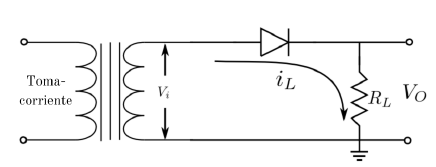
\includegraphics[scale=1]{OndaMedia.png}
	\caption{Circuito para la caracterización de rectificador onda media con un diodo.}
	\label{salida}
\end{figure}

La señal obtenida en el osciloscopio se muestra a continuación

\begin{figure}[h!]
    \centering
    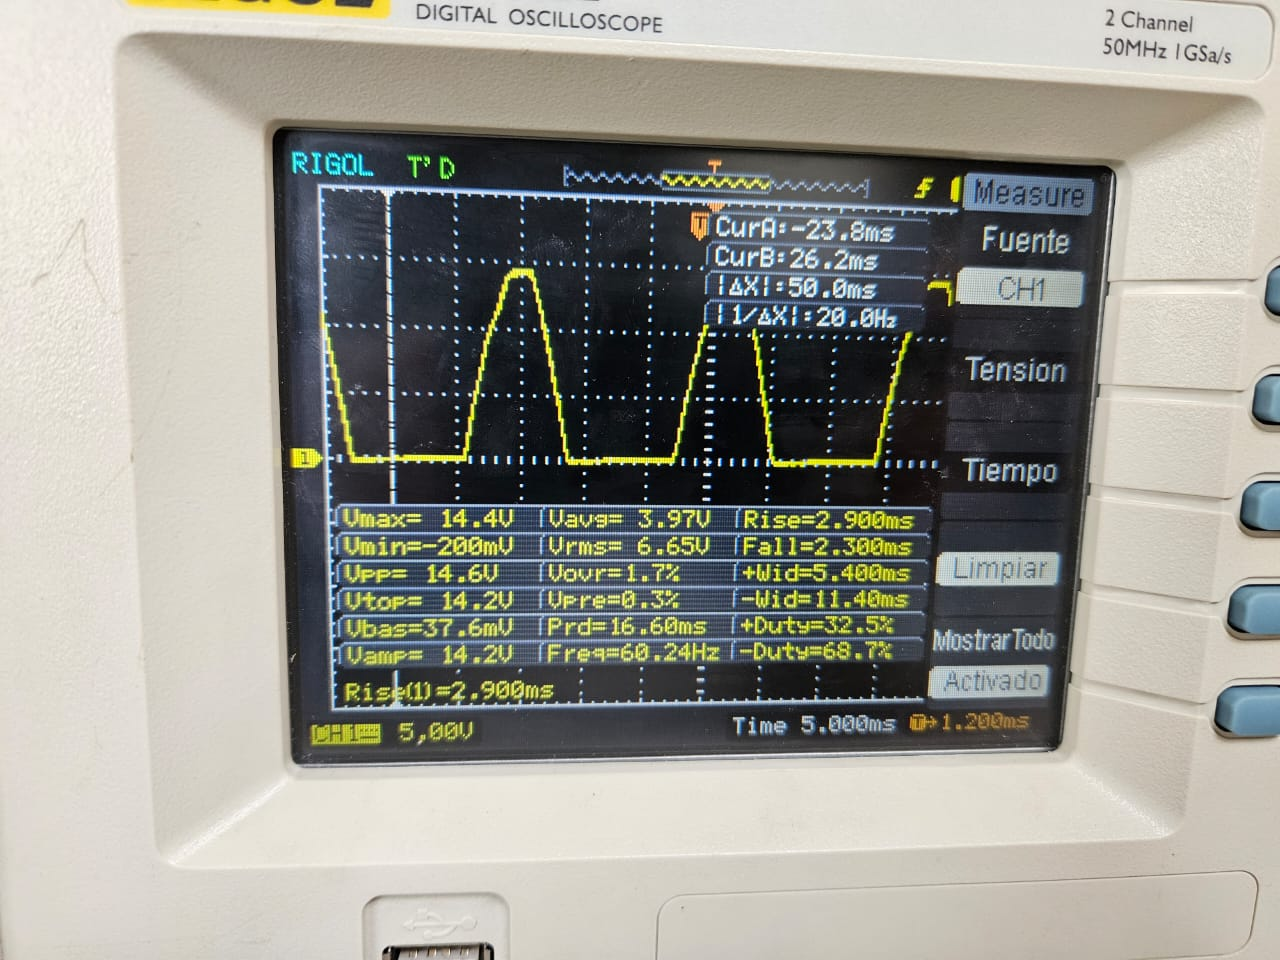
\includegraphics[scale=0.4]{Osc_OndaMedia.jpg}
    \caption{Señal de rectificador de onda media}
    \label{SeñalMedia}
\end{figure}


\subsection{Onda Completa}


\begin{figure}[H]
	\centering
	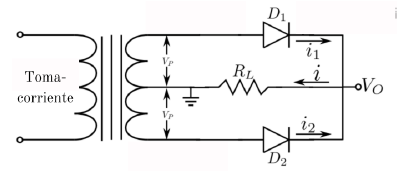
\includegraphics[scale=1]{OndaCompleta2.png}
	\caption{Circuito para la caracterización de rectificador onda completa con dos diodos.}
	\label{fig:enter-label}
\end{figure}

\begin{figure}[H]
	\centering
	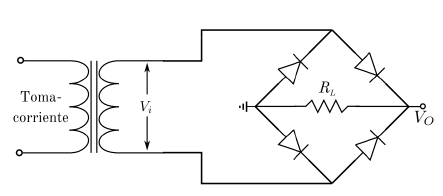
\includegraphics[scale=1]{OndaCompleta4.png}
	\caption{Circuito para la caracterización de rectificador onda completa con cuatro diodos}
	\label{fig:enter-label}
\end{figure}



\subsection{Rizado de Filtrado}

\begin{figure}[h!]
	\centering
	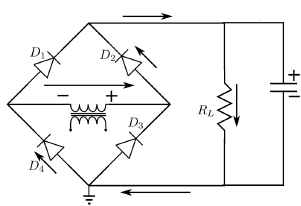
\includegraphics[scale=1]{OndaCapacitorFiltrado.png}
	\caption{Circuito para la caracterización de rectificador onda completa con cuatro diodos y capacitor de filtrado}
	\label{fig:enter-label}
\end{figure}



\begin{equation}
	V_{CC}-(i_CR_{C})-V_{CE}=0
\end{equation}
Despejando para $i_C$:

\begin{equation}
	i_C=\frac{ V_{CC}-V_{CE}}{R_{C}}
\end{equation}




\section{Conclusiones}
\begin{itemize}
	\item








\end{itemize}

\begin{thebibliography}{9}

\end{thebibliography}

\end{document}